\begin{figure}
        \centering
        \begin{subfigure}[b]{0.7\textwidth}
                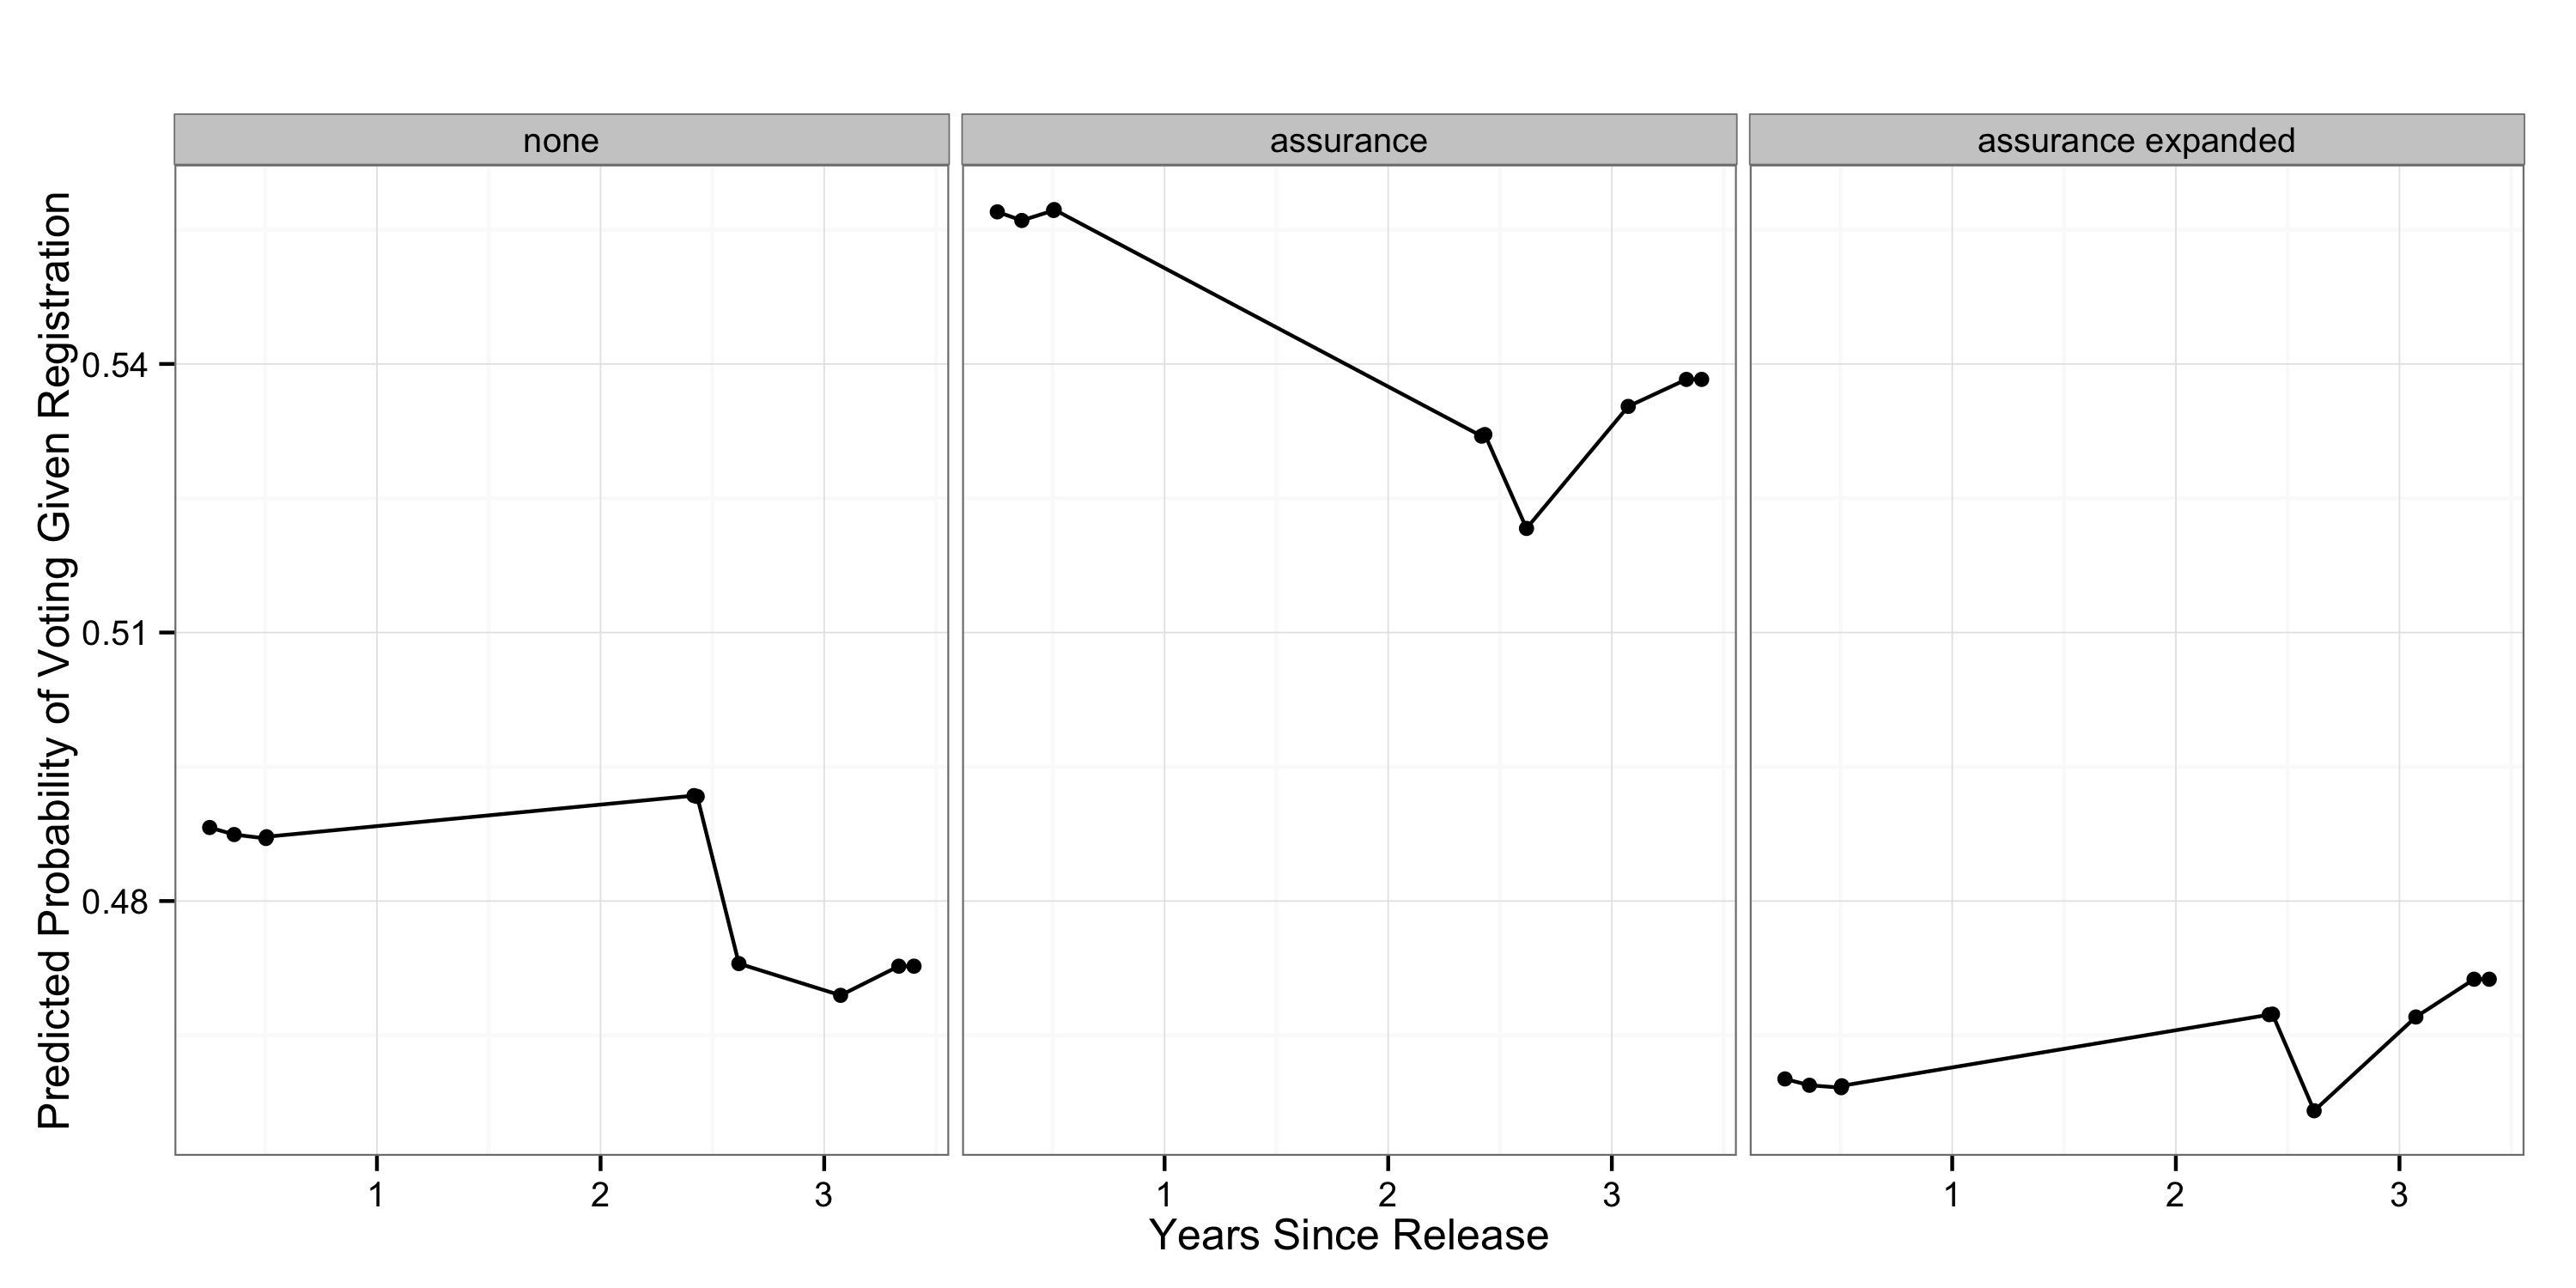
\includegraphics[width=\textwidth]{figures/pd_int_cond_vote.png}
                \caption{Two way partial dependence for interaction detection in the prisoners example. The panels of the figure correspond to the three experimental groups, the line in each panel displays the relationship of years after release with the predicted probability to vote after registration, conditional on the experimental group. }
                \label{fig:int_prison}
        \end{subfigure}%
        ~ %add desired spacing between images, e. g. ~, \quad, \qquad, \hfill etc.
          %(or a blank line to force the subfigure onto a new line)

        \begin{subfigure}[b]{0.7\textwidth}
                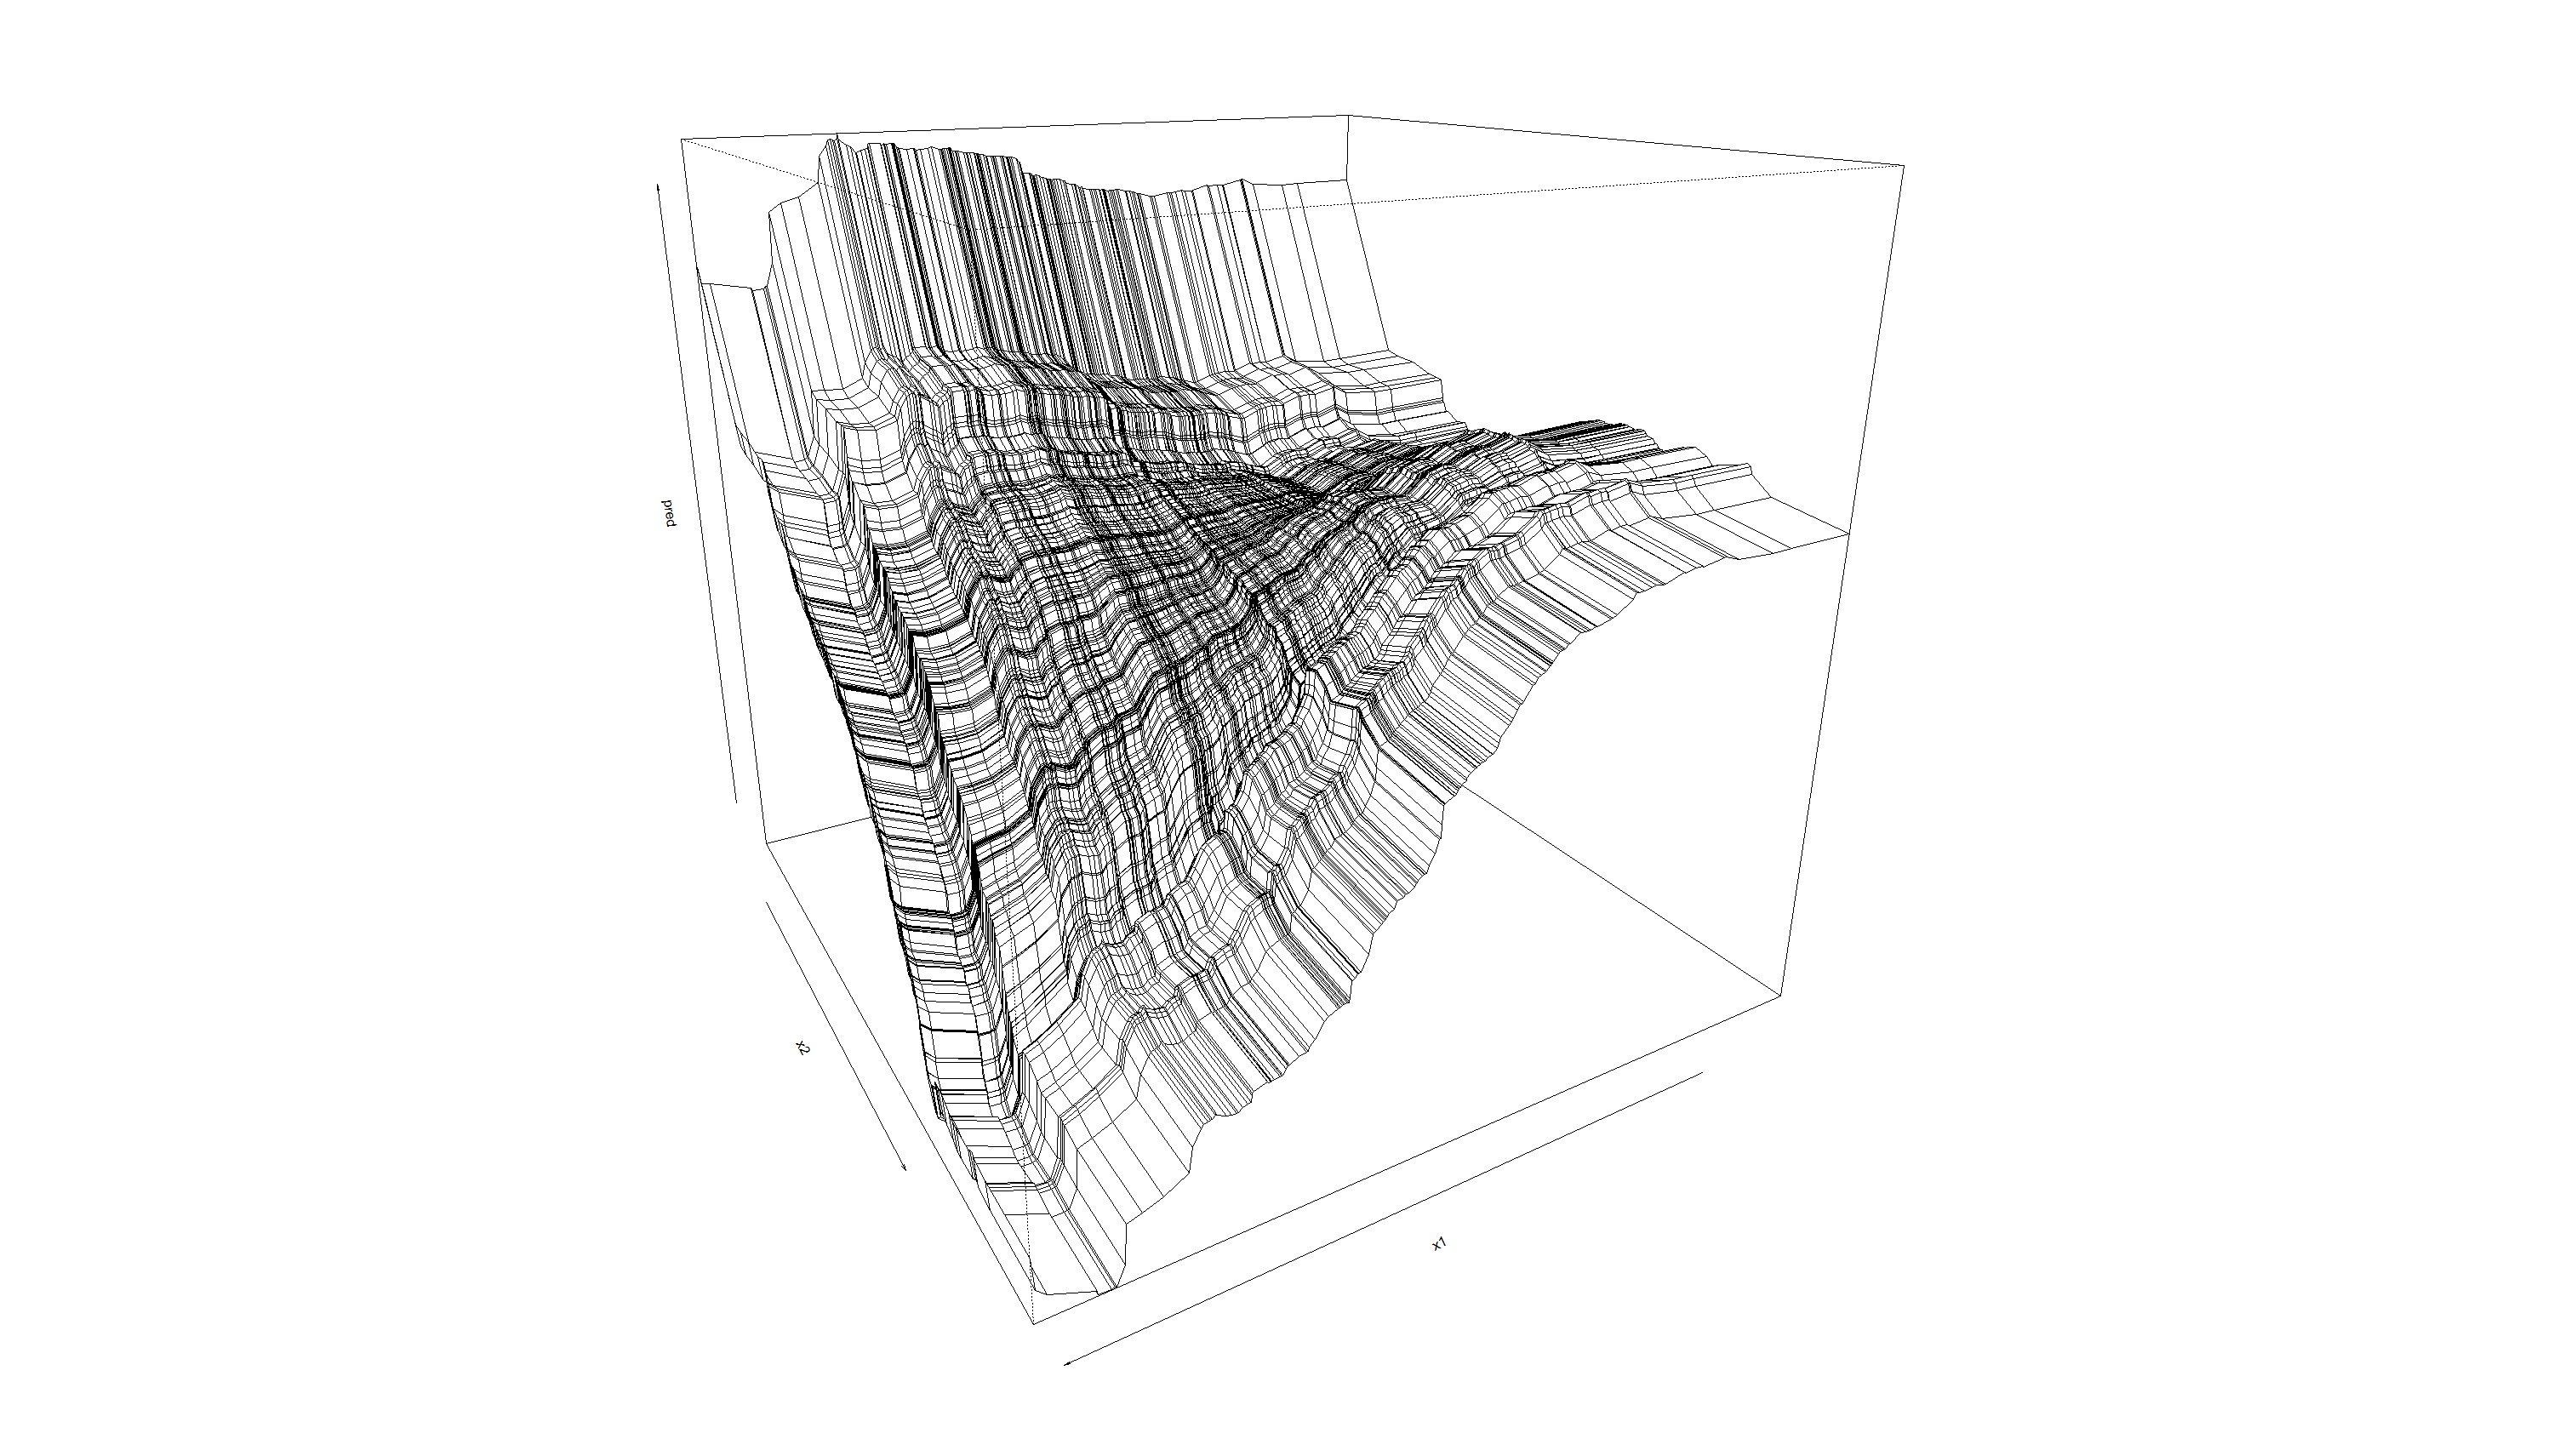
\includegraphics[width=\textwidth]{figures/interaction.png}
                \caption{Two way partial dependence for interaction detection in simulated data set. Each intersection of the grid represents a value pair for the variables $x_1$ and $x_2$. The height of the plot represents the average prediction from the partial dependence algorithm.}
                \label{fig:int_3d}
        \end{subfigure}
        \caption{Interaction detection with partial dependence. Visualization by faceting and with 3-D plotting.}
        \label{fig:interaction}
\end{figure}
